\documentclass[elementsmain.tex]{subfiles}
\begin{document}
\section{Example Subspaces: Null Spaces}

At this point, we have identified several different kinds of subsets of $\R^n$ which are useful from a linear algebra point of view: affine subsets, hyperplanes, and now subspaces. We now start to sort out the relationships between these three things. Along the way, we will introduce one of the primary ways to generate examples of subspaces: as the null space of a matrix.

Let's begin by looking at the connection between the idea of an affine subset and the idea of a subspace.

\begin{theorem} Let $\mathcal{S}$ be a subspace of $\R^n$. Then $\mathcal{S}$ is an affine subset of $\R^n$.
\end{theorem}

\begin{proof}
Note that if $\mathcal{S}$ is the trivial subspace $\mathcal{S}= \{0\}$, then it has only one vector in it, so there is nothing to check in the definition of affine subset. So we may proceed by assuming that $\mathcal{S}$ has at least two vectors in it.

Let $u$ and $v$ be any two elements of the subspace $\mathcal{S}$. To show that $\mathcal{S}$ is an affine subset of $\R^n$, we must show that the whole line through $u$ and $v$ is also in $\mathcal{S}$.

But any point on the line through $u$ and $v$ can be written in the form 
\[
u + t(v-u) = (1-t) u + t v,
\]
where $t$ is some real number. So we see that such a point is a linear combination of $u$ and $v$. Since $\mathcal{S}$ is a subspace, this linear combination is also in $\mathcal{S}$. Therefore, $\mathcal{S}$ is also an affine subset of $\R^n$.
\end{proof}


\begin{theorem}\label{thm:13-2} Let $\mathcal{A}$ be an affine subset of $\R^n$ which contains the origin. Then $\mathcal{A}$ is a subspace of $\R^n$.
\end{theorem}

\begin{proof} Let $u$ and $v$ be two elements of $\mathcal{A}$. We must show that every linear combination $au+bv$ is also an element of $\mathcal{A}$. \\

Our approach will be to do this in stages. First we will find a line of points in $\mathcal{A}$, and then we will ``sweep out'' most of the linear combinations by taking lines through the origin and the points on this line. Finally, we will patch up the rest of the linear combinations by showing that the missing set (which will be a line) can be covered, too.

\noindent
\textbf{Step 1: $a+b\neq 0$}

First note that the line $\ell'$ which passes through $u$ and $v$ is part of $\mathcal{A}$, because $\mathcal{A}$ is an affine subset. Therefore, each point of the form $u + t(v-u)$ is in $\mathcal{A}$. In particular, if we choose $t = \dfrac{b}{a+b}$, we see that 
\[
w = u + t (v-u) = u + \dfrac{b}{a+b}(v-u) = \dfrac{a}{a+b} u + \dfrac{b}{a+b} v
\]
is an element of $\mathcal{A}$. 

Since $0$ is in $\mathcal{A}$, too, the line through $0$ and $w$ lies in $\mathcal{A}$. Therefore, each vector of the form $\lambda w$ is in $\mathcal{A}$.
If we choose $\lambda = a+b$, we see that 
\[
(a+b) w = \left( \dfrac{a}{a+b} u + \dfrac{b}{a+b} v \right) = au + bv
\]
is an element of $\mathcal{A}$. This completes the proof in the case that $a+b\neq 0$.

\begin{figure}[h]
\centering
\begin{tikzpicture}
\draw (-2.5,0) -- (6,0);
\draw[fill] (0,0) circle[radius=0.05]  node[below left] {$0$};
\draw[->,thick] (0,0) -- (2,-2) node[right] {$-2u$};
\draw[->,thick] (0,0) -- (-1,1) node[below left] {$u$};
\draw[->,thick] (0,0) -- (2,1) node[below right] {$v$};
\draw[->,thick] (0,0) -- (4,2) node[below right] {$2v$};
\draw (-2.5,1) -- (6,1) node[above left] {$\ell$};
\draw[->,thick] (0,0) -- (2,4) node[left] {$au+bv$};
\draw[->,ultra thick] (0,0) -- (.5,1);
\draw[->,dashed] (-.5,2.5) node[above] {$w = u+\dfrac{b}{a+b}(v-u)$} -- (.2,.55);
\draw[->,thick] (0,0) -- (1,-1) node[left] {$-u$}; 
\draw[->,thick] (0,0) -- (3,0) node[below right] {$v-u$};
\draw (1.5,-3) -- (5,4) node[left] {$\ell'$};
\end{tikzpicture}
\caption{The geometry in our argument for Theorem \ref{thm:13-2}.}
\label{fig:13-plane-sweep}
\end{figure}

You should note that we have definitely shown that $-2u = -2u + 0v$ and $2v = 0u+2v$ are elements of $\mathcal{A}$.

\noindent
\textbf{Step 2: $a+b=0$.}

Now suppose $a+b=0$. Then $au+bv = b (v-u)$. We will want to show that $v-u$ is an element of $\mathcal{A}$, and then the same reasoning as above about the line through this point will show that $au+bv = b(v-u$ lies in $\mathcal{A}$. 

Since $-2u$ and $2v$ are elements of $\mathcal{A}$, so is the line which passes through them. So we see that every point of the form
\[
-2u + s (2v-2u) = (-2-2s) u + (2s) v 
\]
lies in $\mathcal{A}$. But if we choose $s=1/2$, this tells us that $v-u$ is in $\mathcal{A}$.

Putting everything together, we get that all of the linear combinations $au+bv$ are elements of $\mathcal{A}$, so $\mathcal{A}$ is a subspace.
\end{proof}

We have already seen that there is a connection between hyperplanes and affine subspaces. So it is natural to suspect that we can make a connection between hyperplanes and subspaces, too. That is the subject of the next few results. We will give the statements here, and leave it for the exercises to give arguments. 

\begin{remark}[Notation for Hyperplanes] For a non-zero vector $N\in \R^n$ and a scalar $c\in \R$, we will use the following notation for the hyperplane with normal vector $N$ and level $c$:
\[
\mathcal{H}_{N,c} = \{  X \in \R^n \mid N\cdot X = c \}.
\]
That is, $\mathcal{H}_{N,c}$ will represent the set of all possible vectors $X$ which are solutions to the linear equation $N\cdot X = c$.

Remember that $\mathcal{H}_{N,c}$ contains the zero vector (the origin) exactly when $c=0$.
\end{remark}


\begin{theorem}\label{thm:13-hyp-subs} The hyperplane $\mathcal{H}_{N,c}$ in $\R^n$ is a subspace if and only if $c=0$. That is, a hyperplane $\mathcal{H}_{N,c}$ is a subspace if and only if it contains the origin.
\end{theorem}

\begin{proof} You will work out a proof of this in Exercises \ref{ex:13-pf-thm-hyp-subs1} and \ref{ex:13-pf-thm-hyp-subs2}.
\end{proof}

\begin{theorem} A finite intersection of hyperplanes is a subspace if and only if that intersection contains the origin. That is, the intersection of hyperplanes $\mathcal{H}_{N_k,c_k}$ is a subspace if and only if each of the $c_k$'s is zero.
\end{theorem}

\begin{proof}
Apply Theorem \ref{thm:13-hyp-subs} several times.
\end{proof}


If we recall that the intersection of a finite number of hyperplanes is an affine subspace, we can restate this last result in a way that makes it a special case of Theorem \ref{thm:13-2}.

\begin{corollary} The affine subset of $\R^n$ which is the set of solutions to a homogeneous system of $m$ linear equations in $n$ unknowns is a subspace of $\R^n$.
\end{corollary}

Of course, we have already seen that a homogeneous system of $m$ linear equations in $n$ unknowns can be rewritten as a matrix-vector equation of the form $Ax=0$, where $A$ is the $m\times n$ matrix of coefficients. This motivates the following definition.

\begin{definition}[Null Space of a Matrix]
Let $A$ be an $m\times n$ matrix. The \emph{null space of $A$} is the subspace of $\R^n$ which consists all solutions to the associated homogeneous equation $Ax=0$. That is, 
\[
\mathrm{null}(A) = \{ x \in \R^n \mid Ax=0 \}.
\]
\end{definition}


\begin{definition}[Annihilator Matrix]
Let $\mathrm{S}$ be a subspace of $\R^n$. A matrix $A$ is called \emph{an annihilator matrix for $\mathcal{S}$} when $S=\mathrm{null}(A)$.
\end{definition}

Usually, a subspace has many different annihilator matrices.


\clearpage

\subsection*{Exercises}

\begin{exercise} Restate the definition of the null space of a matrix in a way that involves a linear-combination equation.
\end{exercise}

\begin{exercise}
Write down an example of subspace $\mathcal{T}$ which is just a line in $\R^2$ through the origin. Find two different annihilator matrices for $\mathcal{T}$.
\end{exercise}


\begin{exercise}
Find an annihilator matrix for the subspace $\mathcal{S}_1$ of $\R^3$ given below.
\[
\mathcal{S}_1 = \{ a u + b v \mid a,b \in \R^3 \},
\]
where
\[
u = \begin{pmatrix} -2\\1\\0 \end{pmatrix}, \quad 
v = \begin{pmatrix} -1 \\ 0 \\ 1 \end{pmatrix}.
\]
You can take for granted that $\mathcal{S}_1$ is a subspace.
\end{exercise}

\begin{exercise}
Find an annihilator matrix for the subspace $\mathcal{S}_2$ of $\R^3$ given below.
\[
\mathcal{S}_2 = \{ a u + b v \mid a,b \in \R^3 \},
\]
where
\[
u = \begin{pmatrix} 1\\1\\1 \end{pmatrix} \quad 
v = \begin{pmatrix} 1\\2\\0 \end{pmatrix}.
\]
You can take for granted that $\mathcal{S}_2$ is a subspace.
\end{exercise}


%\begin{exercise}
%find an annihilator matrix for a span of one vector in $\R^3$
%\end{exercise}

\begin{exercise}
Can you describe the null space of this matrix $A$?
\[
A = \begin{pmatrix} 1 & 2 & 0 & 0 & 2 \\ 0 & 0 & 1 & 0 & 9 \\
0 & 0 & 0 & 1 & -2 \\ 0 & 0 & 0 & 0 & 0 \end{pmatrix}
\]
\end{exercise}


\begin{exercise}\label{ex:13-pf-thm-hyp-subs1}
Give an argument in support of Theorem \ref{thm:13-hyp-subs} in the following manner: Assume that $u$ and $v$ are two elements in the hyperplane $\mathcal{H}_{N,0}$, then give a reason why $au+bv$ must also be an element of $\mathcal{H}_{N,0}$.
\end{exercise}

\begin{exercise}\label{ex:13-pf-thm-hyp-subs2}
Make an example of a hyperplane $\mathcal{H}_{N,c}$ in $\R^2$ where $c\neq 0$. Use the geometry your example to show why the hypothesis $c=0$ is necessary by showing why $\mathcal{H}_{N,c}$ fails to be a subspace on both conditions of being a subspace.
\end{exercise}

%\begin{exercise}
%prove theorem \ref{thm:13-fin-int-hyp-subs}--- use friendlier term
%\end{exercise}

%\begin{exercise}
%show c=0 breaks theorem
%\end{exercise}

\begin{exercise} Make a diagram that helps to organize the logical connections between the ideas of affine subset, hyperplane, and subspace, given what we know right now. Is there anything else we should figure out?
\end{exercise}

\clearpage
\end{document}